\begin{figure}[!htbp]
  \centering
  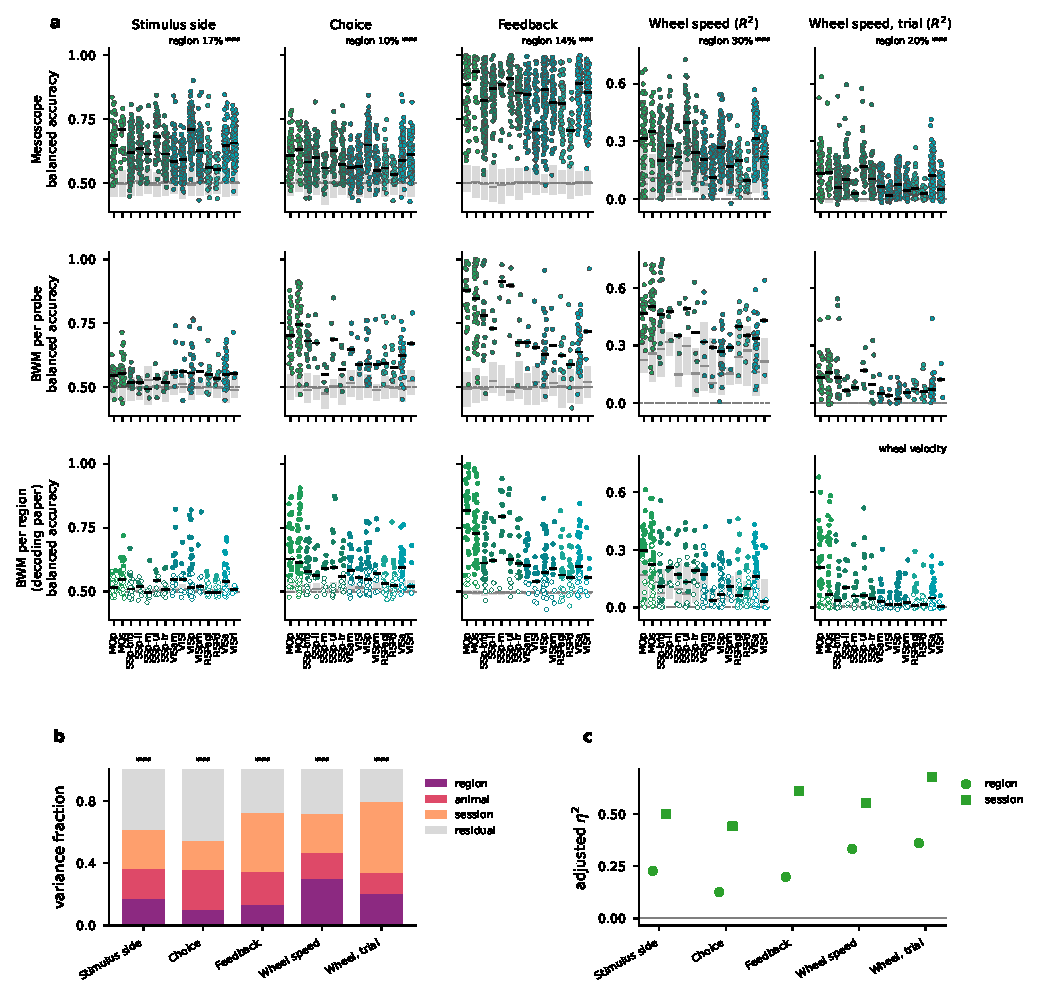
\includegraphics[width=\linewidth,height=0.8\textheight,keepaspectratio]{figures/region_variance.pdf}
  \caption{\textbf{Variance of decoding across regions and sessions (all neurons).} The 15 regions with $\geq$3 mesoscope sessions and BWM probes. Methods: \emph{Region and session variance}. \textbf{a} Scores per region (columns ordered as in the Allen structure tree; Allen colours; bar: median; dashed: chance; grey band and line: 5--95th percentile and median of the baseline; for trial-specific wheel speed the shuffle baseline lies at $R^2 \approx 0$ and is hidden by the dashed line). Top: mesoscope, one dot per session and region from all its neurons there (149 sessions, 12 animals); baseline: shuffle control. Middle: BWM, one dot per probe from all its isocortex units, placed in the region where it enters the brain (198 probes, 93 animals; the majority region of its superficial units for 66\% of probes); baseline: shuffle control. Bottom: BWM decoding paper, one dot per session and region from the region's units (346 pairs, 263 sessions, 116 animals); filled: $p<0.05$ against pseudo-sessions (21--70\% of dots); baseline: median of the pseudo-session null; wheel velocity in place of trial-specific wheel speed. Y axes shared within balanced accuracy and within $R^2$. Inset, top row: region share of variance from \textbf{b}. \textbf{b} Mesoscope variance fractions from a mixed model, score $\sim$ log $N$ + (1$|$region) + (1$|$animal) + (1$|$session); stars: likelihood-ratio test of the region component. Region: stimulus side 17\%, choice 10\%, feedback 14\%, wheel speed 30\%, wheel, trial 20\%; session plus animal: stimulus side 45\%, choice 44\%, feedback 58\%, wheel speed 41\%, wheel, trial 59\%. \textbf{c} The same question as \textbf{b}, do scores differ more between regions or between sessions, but without a statistical model, using only reshuffling: adjusted $\eta^2$ of region (circles, within sessions) and of session (squares, within regions), 0 = chance. Filled: $p<0.05$.}
  \label{fig:region_variance}
\end{figure}
